 \chapter{Results, Evaluation and Discussion}
\label{chapter4}

This chapter reports the empirical findings of Phases~2 to~10 organised around the four research questions from Chapter~\ref{chapter1}. Phase~9 is reported separately as a validity check on the investigation.

\section{Preliminary validation}
\label{sec:prelim}

The three preliminary gates all passed. Phase~0's integrity suite passed all 12 tests after 2 defects were caught and corrected during development (Appendix~\ref{appendix:phase01}). Phase~1's smoke validation cleared the gate, with all three s0 seeds exceeding the 0.50 win-rate threshold.

Phase~2 ranked the four DQN variants by single-agent win rate against the fixed Base adversary at the noise-free stochasticity level (s0). Rainbow-lite finished first at 0.835, with a 95\% confidence interval (CI) of 0.813--0.856, followed by double DQN at 0.798, vanilla at 0.746 (CI 0.723--0.769), and dueling at 0.724. Rainbow-lite's CI does not overlap vanilla's, so the gap is unlikely to reflect seed variance alone.

Rainbow-lite is also the most stable variant under increasing outcome noise, with its win rate shifting only $+0.005$ from s0 to s2. This is consistent with prioritised experience replay and double-target correction reducing the value instability that affects vanilla under noisy rewards \citep{schaul2016prioritized,vanhasselt2016double}. Rainbow-lite is therefore the leading single-agent substrate candidate, though the single-agent contract cannot establish that the variant remains stable when a second concurrent learner is introduced. That question is taken up in RQ1.

\section{RQ1: What strategic behaviours emerge and how robust are they?}
\label{sec:rq1}

Phase~3 tested four DQN-family variants under concurrent learning at $\alpha = 0$, where two instances of the same variant race each other in a zero-sum setting. Each variant isolates a different candidate cause of MARL pathology, with the analysis below taking each in turn. Collapse rates across nine trials per algorithm are in Table~\ref{tab:phase3-collapse}.

\begin{table}[htbp]
\centering
\small
\caption{Phase 3 collapse rates by algorithm (nine trials per algorithm)}
\label{tab:phase3-collapse}
\begin{tabular}{|l|c|c|c|c|}
\hline
\textbf{Algorithm} & \textbf{s0} & \textbf{s1} & \textbf{s2} & \textbf{Total collapse} \\
\hline
Vanilla DQN   & 1/3 & 1/3 & 2/3 & 4/9 (44\%) \\
Double DQN    & 1/3 & 0/3 & 0/3 & 1/9 (11\%) \\
Dueling DQN   & 1/3 & 1/3 & 2/3 & 4/9 (44\%) \\
Rainbow-lite  & 0/3 & 0/3 & 0/3 & 0/9 (0\%)  \\
\hline
\end{tabular}
\end{table}

The ablation, a controlled comparison where one mechanism at a time is added or removed to isolate its contribution, picks out two distinct failure modes. Double DQN addresses the first and largest source of error. In this domain, early training produces many failed attempts for the trailing agent punctuated by occasional lucky successes at hard zones, which inflates Q-values for the chosen action under vanilla's target computation. Double target correction dampens this by decoupling action selection from evaluation, which removes a real first-order source of error that affects many runs. Double eliminates collapse entirely at s1 and s2, with only one collapse at s0.

Dueling DQN fails to help and has the same collapse rate as vanilla. Its decomposition into state-value and action-advantage works best when actions are near-equivalent in most states. Overtaking is the opposite case, with HOLD versus ATTEMPT and the risk levels within ATTEMPT strongly differentiated in outcome. Dueling can therefore sharpen bad action preferences rather than smooth them, accelerating drift into a bad strategy.

Rainbow-lite closes the remaining gap from 11\% collapse under double to zero. Given the ablation pattern, prioritised experience replay (PER) is the most plausible load-bearing addition, since dueling is neutral here and multi-step returns are not separately isolated. PER addresses a sampling imbalance double cannot reach. Early failed attempts produce $\langle$attempt, negative$\rangle$ transitions that dominate uniform replay and drive $Q(\text{hold})$ above $Q(\text{attempt})$ before exploration can recover. PER up-weights high TD(temporal difference)-error transitions, where TD-error measures the gap between the agent's predicted Q-value for a state-action pair and the value implied by the observed outcome. High-TD-error transitions are disproportionately the rare successes that need to be learned from.

Extending the three vanilla seeds to 750 episodes produced worse collapse rather than recovery, confirming the loop is self-reinforcing within the training horizon \citep{foerster2017stabilising,matignon2012independent}. Rainbow-lite is therefore the substrate for all later phases, with double DQN retained in Phase~3's family ablation and vanilla in Phase~10 as a weak-algorithm comparator.

Where the algorithm prevents collapse, agents develop differentiated zone coverage and opposing risk profiles without any shared coordination. A representative rainbow-lite trial at s2 with 750 episodes reaches a zone differentiation index of 0.405, with Agent~1 focusing on La Source, Les Combes, and Bruxelles with a conservative bias, and Agent~2 covering five zones with an aggressive bias. The pattern is the hawk-dove equilibrium from evolutionary game theory \citep{maynardsmith1973hawkdove}, where two agents settle into complementary aggressive and conservative roles rather than both pursuing the same strategy. It is reached here through iterated best-response learning where each agent adjusts its policy against the current policy of the other \citep{busoniu2008survey}. Collapsed trials produce no such structure. One agent stops competing entirely and the other wins unopposed, matching the degenerate equilibrium predicted for non-cooperative two-agent Q-learning under positional disadvantage \citep{tan1993multiagent}.

Specialisation depends on training budget with high across-seed variance. Some seeds more than double their differentiation index between 500 and 750 episodes, others barely move, and seeds sampled only at 500 episodes span the full range from near-zero to high differentiation (Figure~\ref{fig:phase3-zone-specialisation-growth}). The pattern is budget-sensitive rather than budget-determined. PER needs sufficient zone-specific transitions to produce reliable relative priorities, but initialisation variance also matters for how quickly this stabilises.
\begin{figure}[!htbp]
    \centering
    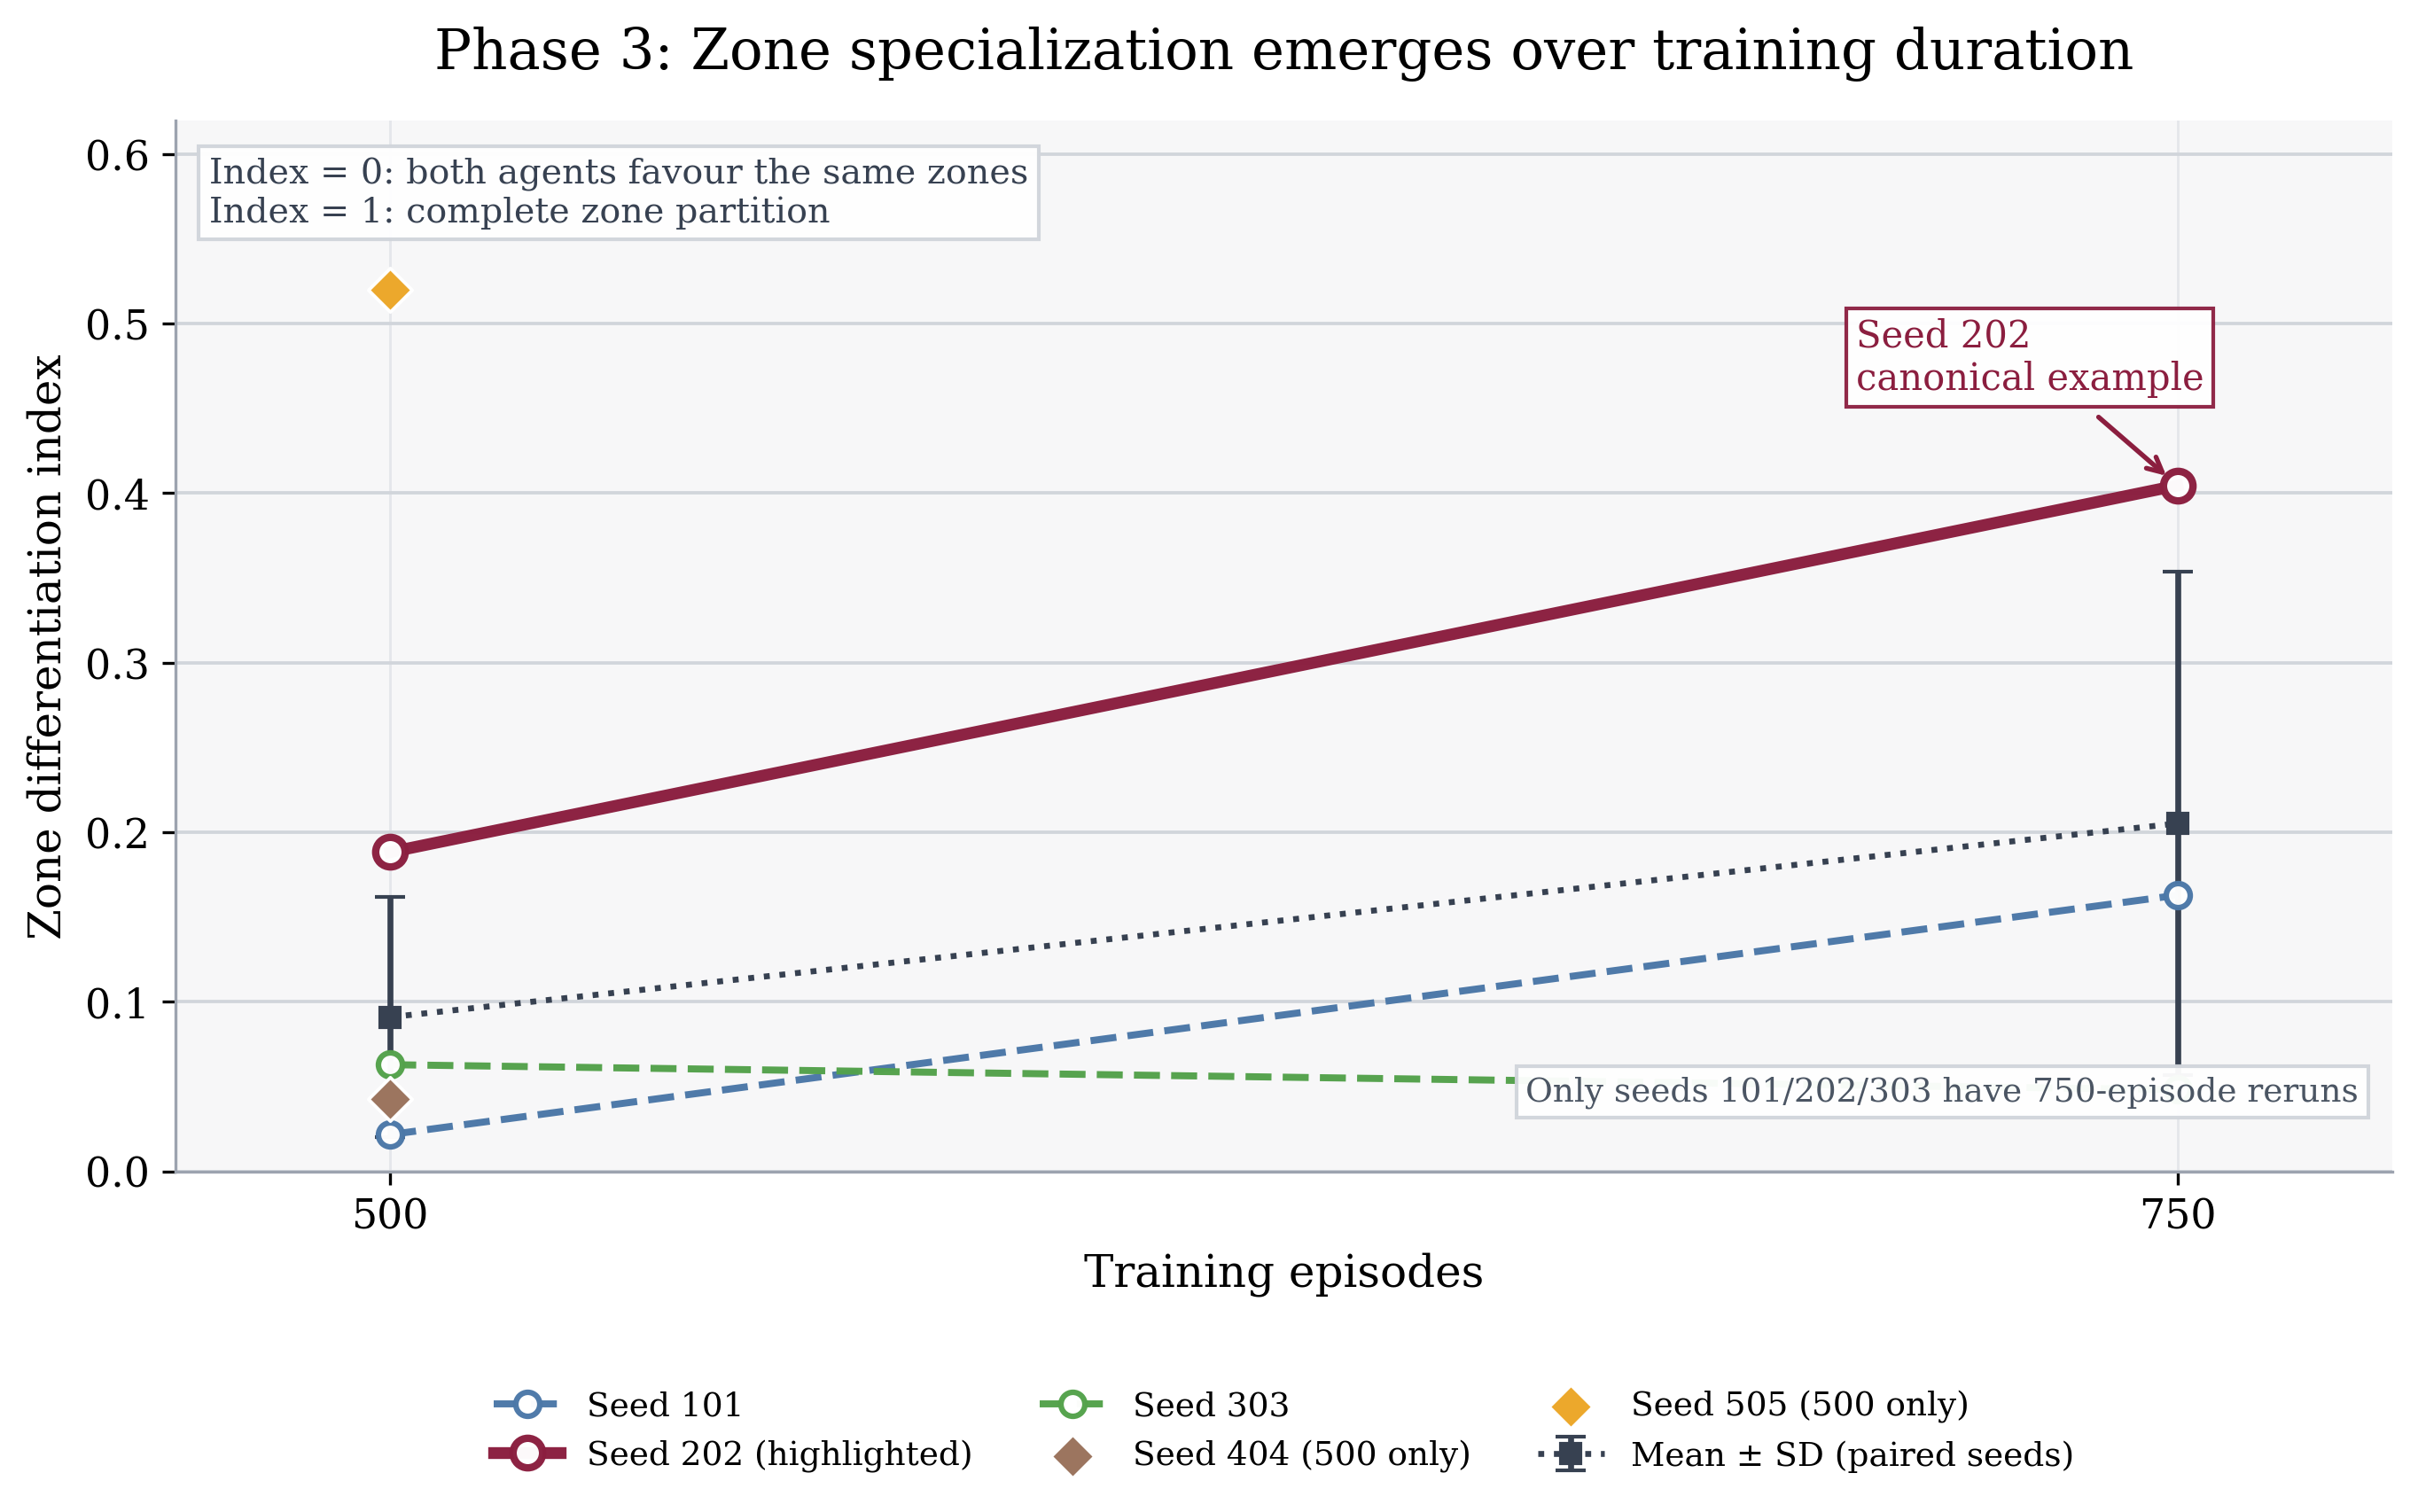
\includegraphics[width=0.88\textwidth]{diagrams/phase3_zone_specialization_growth.png}
    \caption{Zone differentiation growth for rainbow-lite at s2 showing dependence on training budget.}
    \label{fig:phase3-zone-specialisation-growth}
\end{figure}
A crossplay protocol at s2 revealed an 11\%\ point structural bias against the A1 evaluation slot, affecting raw A1 win rates but not collapse classification. After applying the correction, four of five rainbow-lite seeds sit at or above parity, and the apparent A2 dominance at s2 largely dissolves (full arithmetic in Appendix~\ref{appendix:phase3-crossplay}). This supports the evaluation-bias interpretation as opposed to a systematic policy effect. Non-stationarity rather than stochasticity dominates Phase~3. Vanilla and dueling collapse rises from 1/3 at s0 to 2/3 at s2, showing stochasticity accelerates but does not cause collapse \citep{foerster2017stabilising}.

\textbf{RQ1 answer.} H1 is confirmed for collapse-resistant algorithms. In all nine rainbow-lite trials and eight of nine double DQN trials, non-degenerate asymmetric behaviour emerges without explicit coordination. Rainbow-lite produces clean hawk-dove risk partitioning as the canonical case, while double DQN's non-collapsed trials produce weaker forms of asymmetry including zone-avoidance patterns and wrong-zone fixation. Vanilla and dueling collapse in 44\%\ of trials and produce no strategic structure at all, so H1 holds only where the algorithm survives the non-stationarity challenge. Specialisation depends jointly on training budget and initialisation variance rather than budget alone, and non-stationarity from concurrent learning is the dominant challenge as opposed to environmental stochasticity.

\section{RQ2: How does incentive structure alter strategy?}
\label{sec:rq2}

Phase~4 ran the $\alpha$ sweep in the two-agent zero-sum game. Collapse is low at $\alpha \le 0.5$, sharp between $\alpha = 0.5$ and $\alpha = 0.75$, and complete at $\alpha = 1.0$ (Table~\ref{tab:phase4-collapse}, Figure~\ref{fig:phase4-collapse-vs-alpha}). At $\alpha \ge 0.75$ the cooperative reward term dominates the individual gradient, turning successful overtakes into net penalties and driving both agents to passivity \citep{claus1998dynamics}. The exact 8/9 figure at $\alpha = 0.75$ is numerically imprecise under the three-seed design, though the qualitative pattern is robust.

\begin{table}[htbp]
\centering
\small
\caption{Phase 4 collapse rates by $\alpha$ in two-agent zero-sum game (9 trials per $\alpha$)}
\label{tab:phase4-collapse}
\begin{tabular}{|c|c|c|}
\hline
\textbf{$\alpha$} & \textbf{Collapse rate} & \textbf{Competitive trials} \\
\hline
0.00 & 0/9 (0\%)   & 100\% \\
0.25 & 1/9 (11\%)  & 89\% \\
0.50 & 1/9 (11\%)  & 89\% \\
0.75 & 8/9 (89\%)  & 11\% \\
1.00 & 9/9 (100\%) & 0\%  \\
\hline
\end{tabular}
\end{table}

Two secondary patterns within the threshold qualify how $\alpha$ acts rather than just where it acts. Zone convention formation is non-monotonic, peaking at $\alpha = 0.25$ and declining thereafter, and stochasticity's role inverts across the threshold from stabilising at low $\alpha$ to destabilising at high $\alpha$ (Appendix~\ref{appendix:phase4-patterns}). Together these show $\alpha$ changing the type of equilibrium rather than the strength of a single one. Low $\alpha$ produces competitive convention with differentiated zone coverage. High $\alpha$ produces an unstable passive equilibrium where both agents learn to hold.
\begin{figure}[!ht]
    \centering
    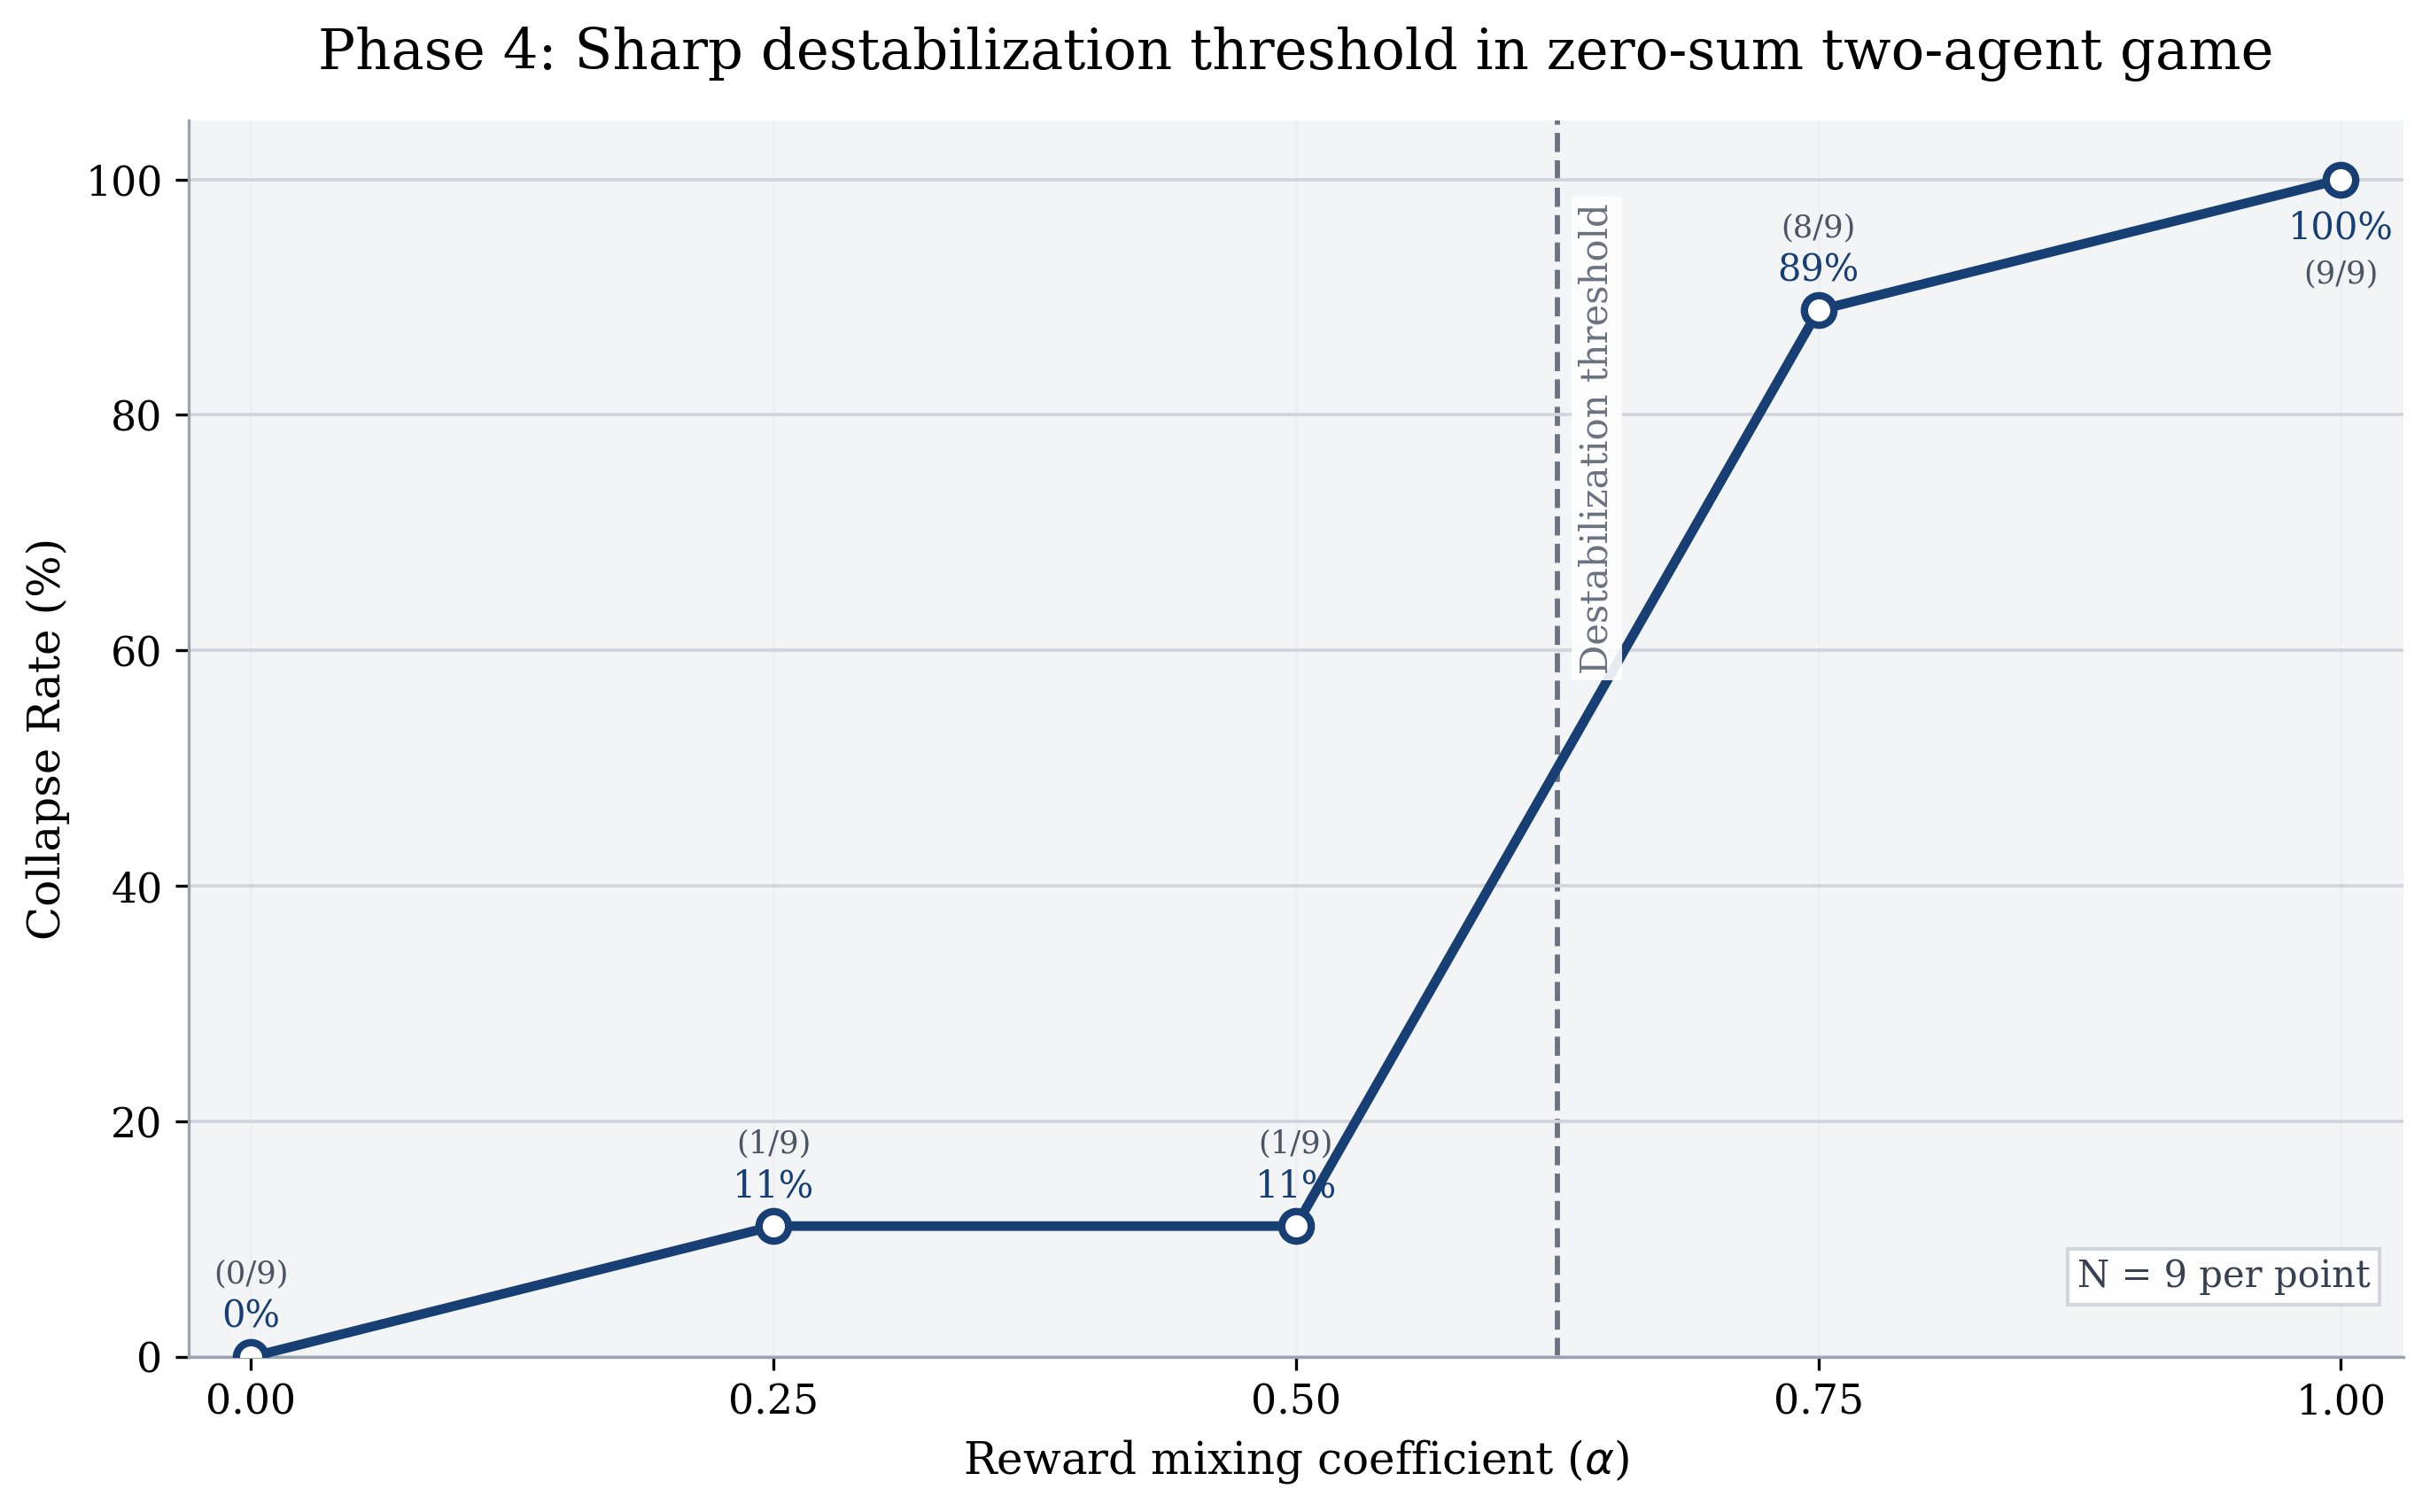
\includegraphics[width=0.88\textwidth]{diagrams/phase4_collapse_vs_alpha.png}
    \caption{Collapse rates by $\alpha$ in the two-agent zero-sum game.}
    \label{fig:phase4-collapse-vs-alpha}
\end{figure}
Phase~5 ran the same sweep in the minimal non-zero-sum configuration of two DQN agents plus one Base adversary. The curve is fundamentally different (Table~\ref{tab:phase5-results}). Collapse disappears at all $\alpha$ values. Joint beat-base rate follows an inverted-U peaking at $\alpha = 0.75$, rising from 0.310 at $\alpha = 0$ to 0.567 at $\alpha = 0.75$, an 83\%\ improvement. There is no destabilisation threshold here, only a performance optimum. Full cooperation at $\alpha = 1.0$ stays active but becomes higher-variance and less consistent than $\alpha = 0.75$, confirming that 0.75 is a genuine optimum as opposed to a saturating plateau.

\begin{table}[htbp]
\centering
\small
\caption{Phase 5 joint beat-base rate by $\alpha$ in three-agent non-zero-sum game (9 trials per $\alpha$)}
\label{tab:phase5-results}
\begin{tabular}{|c|c|c|c|}
\hline
\textbf{$\alpha$} & \textbf{Joint beat-base} & \textbf{Change from $\alpha=0$} & \textbf{Collapse rate} \\
\hline
0.00 & 0.310 & baseline & 0\% \\
0.25 & 0.294 & $-5\%$   & 0\% \\
0.50 & 0.433 & $+40\%$  & 0\% \\
0.75 & 0.567 & $+83\%$  & 0\% \\
1.00 & 0.436 & $+41\%$  & 0\% \\
\hline
\end{tabular}
\end{table}

Cooperation has a minimum effective dose. At $\alpha = 0.25$ joint beat-base drops 5\%\ below the $\alpha = 0$ baseline, so weak sharing is worse than none. Meaningful benefit starts at $\alpha = 0.5$ and peaks at $\alpha = 0.75$. Small cooperative signals plausibly introduce noise into the individual gradient without inducing role partitioning, leaving agents with weakened incentive signal and no coordination benefit. Above $\alpha = 0.5$ the signal is strong enough to drive complementary role development.

The mechanism behind the cooperative gain is redistributive rather than uniform. Agent~2 rises from 63\%\ beat-base at $\alpha = 0$ to 78\%\ at $\alpha = 0.75$, while Agent~1's rate changes less. The joint metric moves because the floor rises. This is consistent with cooperative incentive functioning as a mechanism that closes within-team performance gaps rather than lifting both agents in parallel \citep{hughes2018inequity}. Strategy and performance metrics also separate. Zone differentiation peaks at low $\alpha$, risk differentiation increases with $\alpha$, and joint performance peaks at $\alpha = 0.75$.

\textbf{RQ2 answer.} H2 predicted a sharp threshold above which shared reward destabilises learning, with the same threshold marking the onset of performance decline in non-zero-sum settings. The zero-sum part is confirmed at the $\alpha = 0.5$ to $\alpha = 0.75$ boundary, with a non-monotonic convention-formation pattern below and a stochasticity inversion across it. The non-zero-sum part is also confirmed. The destabilisation disappears, replaced by an inverted-U performance curve with a minimum effective dose between $\alpha = 0.25$ and $\alpha = 0.5$, an optimum at $\alpha = 0.75$, and decline beyond, with gains driven by lifting the weaker agent. H2 therefore holds in both parts because $\alpha$ changes the type of equilibrium across game structures: zero-sum above threshold produces an unstable passive equilibrium, while non-zero-sum produces an inverted-U with a performance optimum at the threshold. Whether cooperative advantage survives at larger agent counts is addressed in RQ3.
\section{RQ3: Does shared incentive produce genuine cooperative advantage at scale?}
\label{sec:rq3}

RQ2 established that cooperative advantage exists in the minimal non-zero-sum setting and produces a sharp performance optimum at $\alpha = 0.75$. RQ3 tests whether this survives scaling, and the failure mode that emerges is importantly different from anything in RQ2. Across Phases 6, 7, and 8, collapse remains at zero in all 99 trials. The system stays active at scale. What disappears is the cooperative surplus. Agents still race and still respond to $\alpha$, but shared reward stops producing within-team co-improvement.

Phase~6 scaled to four DQN agents in two teams of two plus the Base adversary. Every tested form of cooperation degrades performance. At symmetric $\alpha = 0.75$, joint beat-base drops 31\% from the competitive baseline (Table~\ref{tab:phase6-results}), and the asymmetric condition shows the cooperative team losing both to baseline and to a competitive opponent directly. The Base adversary benefits from this degradation, moving from an average finishing position of 3.315 to 2.956 under symmetric $\alpha = 0.75$. Curriculum scheduling restores Base to its original position, confirming that cooperative-team caution opens space the Base heuristic can exploit.

\begin{table}[htbp]
\centering
\small
\caption{Phase 6 mean team both-beat-base rate by team $\alpha$ condition (9 trials per condition)}
\label{tab:phase6-results}
\begin{tabular}{|l|c|c|}
\hline
\textbf{Condition} & \textbf{Mean team both-beat-base} & \textbf{Change from 0 vs 0} \\
\hline
Team A $\alpha=0.0$ vs Team B $\alpha=0.0$   & 0.350 & baseline \\
Team A $\alpha=0.5$ vs Team B $\alpha=0.5$   & 0.306 & $-12\%$ \\
Team A $\alpha=0.75$ vs Team B $\alpha=0.75$ & 0.243 & $-31\%$ \\
Team A $\alpha=0.75$ vs Team B $\alpha=0.0$  & 0.291 & $-17\%$ \\
\hline
\end{tabular}
\end{table}

The strongest mechanistic evidence is the persistently negative intra-team position-delta correlation, negative in all 36 Phase~6 trials. Shared reward between teammates never becomes genuine within-team co-improvement at this scale, regardless of $\alpha$ or condition. The root cause is causal dilution of the pairwise cooperative signal. At four agents, each teammate's outcome is influenced by three competitors rather than one, so the pairwise signal carries weaker causal information about the teammate's actions, and updates become noisier \citep{agogino2004unifying}. The observation contract included teammate-aware features that agents could have conditioned on, yet no team-conditional behaviour emerged. Agents have the information needed for coordination but lack the reward signal to learn from it, so the bottleneck is credit assignment rather than observation-space design.

Phase~7 characterised the scaling boundary. The $\alpha = 0.75$ effect moves from $+83\%$ at three agents, to $+5\%$ at four agents (Phase~7A, within noise), to $-31\%$ at five agents (Phase~6), shown in Figure~\ref{fig:phase5to7-cooperative-cliff}. Part of the four-agent drop reflects baseline compounding (one more DQN must beat Base for the joint metric to rise), but $\alpha$ = 0.75 fails to create synergy above this baseline, and individual beat-base rates barely move under $\alpha$ in Phase~7A (52 to 61\%\ band while joint beat-base sits at the independence baseline).

\begin{figure}[htbp]
\centering
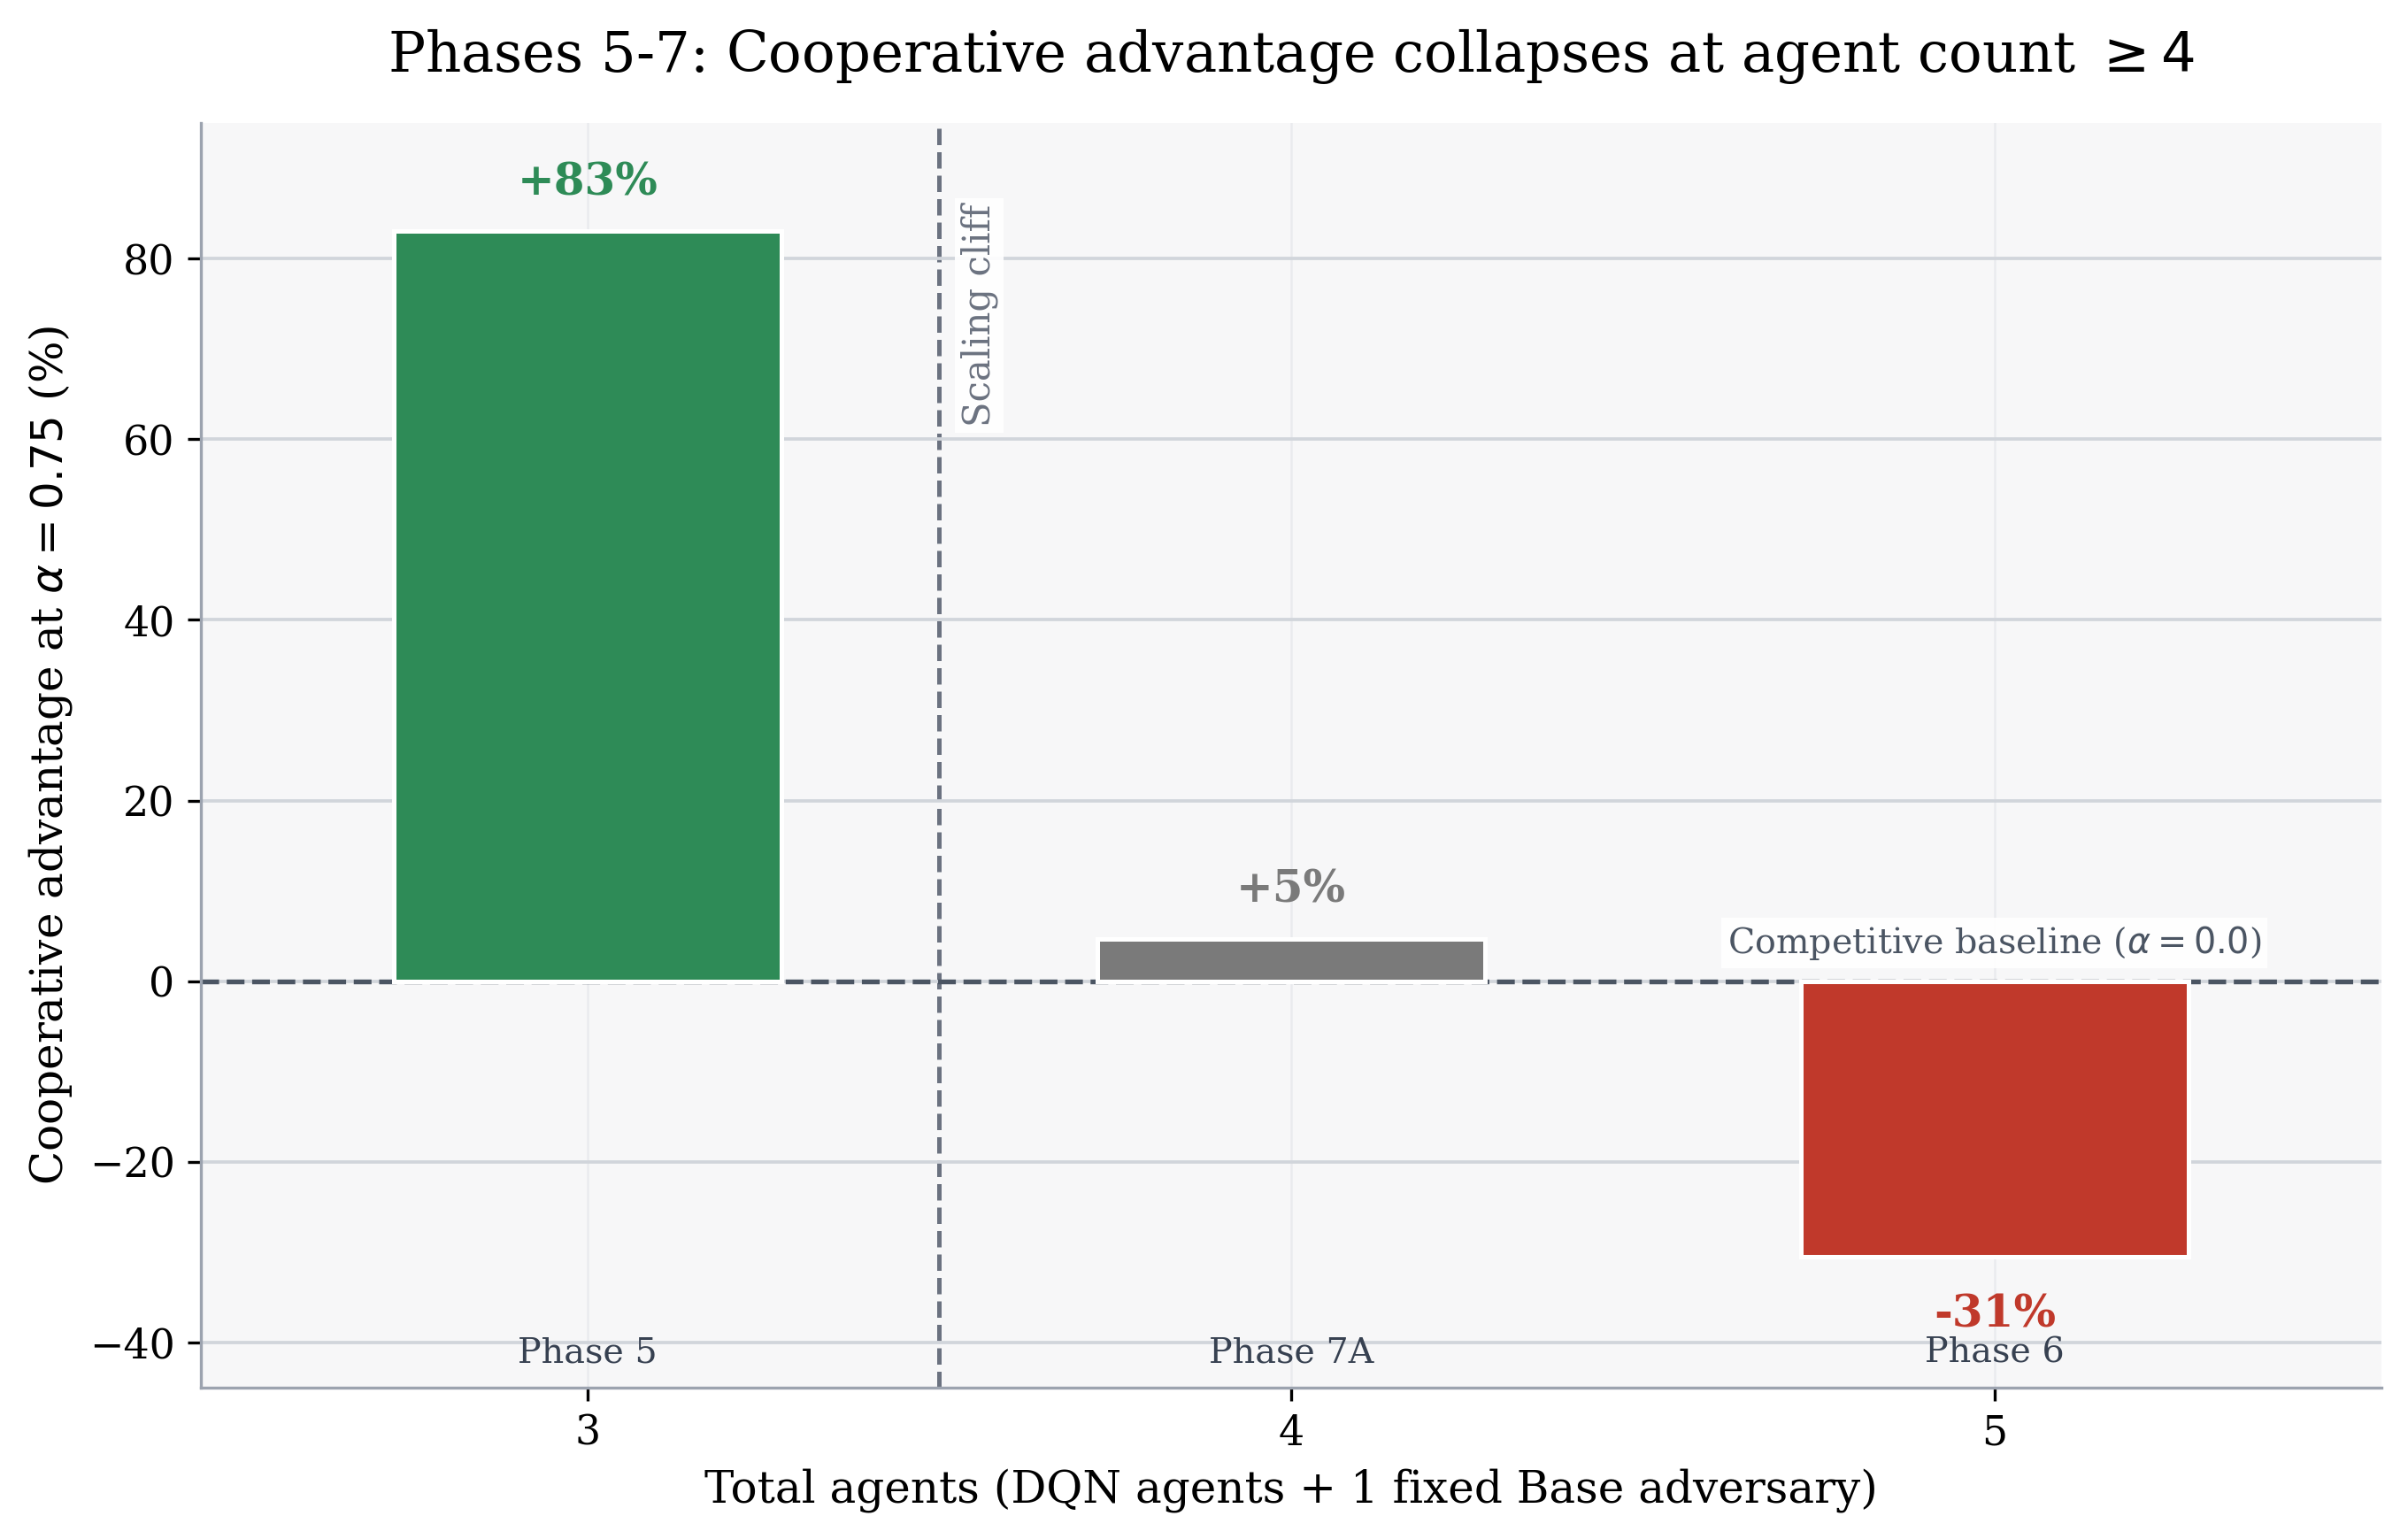
\includegraphics[width=0.75\textwidth]{diagrams/phase5to7_cooperative_advantage_cliff.png}
\caption{Cooperative advantage at $\alpha=0.75$ across agent counts.}
\label{fig:phase5to7-cooperative-cliff}
\end{figure}

Phase~7B tested whether any $\alpha$ value recovers cooperative performance at five agents. Combined with Phase~6 reference points at $\alpha = 0.0$, $0.5$, and $0.75$, the full five-agent team-$\alpha$ sweep is flat at very low $\alpha$ and then downward from $\alpha = 0.25$ onwards (0.350, 0.344, 0.349, 0.315, 0.306, 0.243 at $\alpha = 0.00, 0.10, 0.15, 0.25, 0.50, 0.75$). No $\alpha$ value recovers performance, and the failure is structural rather than parametric. Zone specialisation is necessary but not sufficient for cooperative advantage. At four agents, $\alpha = 0.75$ raised zone differentiation by 63\%\ relative to $\alpha = 0$, yet produced no joint benefit. Attempt rates simultaneously dropped 38 to 64\%\ across zones, so agents responded to the cooperative signal by becoming more cautious rather than coordinating effectively.

Phase~8 tested whether curriculum scheduling recovers cooperative performance. At five agents (Phase~8B) curriculum recovered 69\%\ of the performance loss (joint beat-base rising from 0.243 to 0.318 against the 0.350 baseline), and excessive caution fell 86 to 89\%. At four agents (Phase~8A) curriculum almost eliminated the caution pathology. Curriculum therefore solves the training-order damage that high fixed $\alpha$ causes, yet in no condition does it exceed the competitive baseline. The intra-team correlation becomes even more negative under curriculum ($-0.189$ in Phase~8B), meaning agents improve individually while actively anti-coordinating. Curriculum cleanly separates two failure modes often discussed together \citep{panait2005cooperative, zhao2025maca}. It resolves training-order collapse, where cooperative reward introduced before individual policies stabilise drives agents into passivity. It leaves credit-assignment failure untouched, where overlapping contributions prevent team reward from producing useful per-agent gradients. At four or more agents, reward-level interventions appear insufficient, pointing toward architectural changes such as centralised training with decentralised execution (CTDE) as the next plausible route \citep{rashid2018qmix}.

\textbf{RQ3 answer.} H3 is confirmed. Phase~7B's monotonic downward curve, Phase~8's recovered-but-anti-coordinating outcome, and the persistently negative intra-team correlation across all scaling phases together provide direct evidence. The scaling failure manifests as active anti-coordination as opposed to passive collapse. Agents remain active, $\alpha$ still changes zone allocation, and curriculum restores aggressive play, but none of these changes produce positive within-team coupling. The curriculum clause of H2 finds support in Phase~8's 69\%\ recovery, which is real but insufficient for cooperation. The structural boundary sits at four total agents in this simulator.

\section{RQ4: Can alternative cooperative reward formulations recover advantage at the scaling boundary?}
\label{sec:rq4}

Phase~10 tested the mean-field difference reward approximation (Section~\ref{sec:difference-rewards}) at the four-agent configuration of 3 DQN plus Base, matching the Phase~7A setup where $\alpha$-mixed cooperation had already failed. The test is therefore whether an alternative cooperative formulation recovers advantage at the scaling boundary where $\alpha$ mixing broke down.

The implemented formula has two structural properties that together explain why it cannot produce cooperation. First, the total reward mass is conserved because the sum of teammate rewards equals the sum of their individual deltas, so the formula redistributes credit rather than adding cooperative mass. Second, differentiating any agent's reward with respect to a teammate's delta gives $-1/N$, which is negative. Differentiating with respect to that same agent's own delta gives $(2N-1)/N$, which is amplified relative to the identity. This inverts the cooperative signal as H4 predicted, with own-performance incentive amplified and teammate improvement penalised.

\begin{table}[htbp]
\centering
\small
\caption{Phase 10 joint beat-base rate under difference rewards versus IQL baseline at 4 total agents}
\label{tab:phase10-results}
\begin{tabular}{|l|c|c|}
\hline
\textbf{Condition} & \textbf{Joint beat-base} & \textbf{Change from IQL} \\
\hline
IQL baseline (rainbow-lite, $\alpha=0$) & 0.159 & baseline \\
Difference rewards (vanilla DQN)        & 0.087 & $-45\%$ \\
Difference rewards (rainbow-lite)       & 0.133 & $-16\%$ \\
\hline
\end{tabular}
\end{table}

The empirical result matches the mechanism (Table~\ref{tab:phase10-results}). Difference rewards rank last among the cooperative formulations tested at the four-agent boundary. The original Phase~10 run used vanilla DQN by mistake, producing 0.087 joint beat-base. The corrected rainbow-lite rerun rose to 0.133 but still sits below the 0.159 IQL baseline, confirming the negative result survives removal of the algorithm confound. The relative algorithm effect, comparing vanilla against rainbow-lite under difference rewards, is 31\%. The relative formula effect, comparing IQL against rainbow-lite difference rewards, is 16\%. Algorithm choice therefore remains determining even under a changed reward formula.

The deficit is primarily a within-team coordination failure rather than a failure against Base. Base average position in the corrected rainbow-lite run sits at 2.72, comparable to Phase~7A IQL's 2.69. The joint shortfall reflects the DQN group failing to convert individual competitiveness into joint beat-base success, which is consistent with the structural property analysis. Reward amplification for own-performance keeps individual agents active, but the negative teammate gradient prevents the joint metric from rising.

\textbf{RQ4 answer.} Within the alternative formulation tested here, H4 is confirmed. Only the mean-field difference reward approximation was implemented, and it underperforms all tested four-agent baselines because it redistributes credit without adding cooperative mass, amplifies own-performance incentive, and penalises teammate improvement. The result is about this specific approximation, not Wolpert-Tumer difference rewards in general. A formulation preserving the counterfactual property of the original literature may or may not produce cooperation at this scale, which is a question for future work.

\section{Validity check: LLM semantic baseline}
\label{sec:llm-validity}

Phase~9 (Section~\ref{sec:llm-baseline}) compared trained rainbow-lite against a zero-shot LLM using a fixed hand-authored system template populated automatically from simulator state, across five seeds with 150 races per seed. Rainbow-lite achieved 0.835, 0.839, and 0.840 at s0, s1, s2 respectively, against the LLM's 0.819, 0.827, and 0.837. The gap sits within rainbow-lite's seed variation and is not a substantive performance gap. The two policies reach near-parity through qualitatively different strategies, suggesting the simulator's narrow strategy space admits a short near-optimal policy captured by the prompt template \citep{nagpal2025llm_mca}. Learning is therefore sufficient but not strictly necessary for near-optimal play within this simulator, which qualifies the scope of the MARL findings without invalidating the incentive-structure claims they make. The LLM avoids RL-specific pathologies (Raidillon overuse, suboptimal Stavelot behaviour) that the trained policy still exhibits, suggesting learning captures structure reasoning alone misses. Whether these dynamics hold in richer environments is a question for future work.

\section{Conclusion}
\label{sec:conclusion}

The aim was to characterise how cooperation between self-interested learning agents changes under varying incentive alignment, agent count, and reward formulation, and to identify the mechanism wherever cooperation fails. Both halves are answered. The characterisation is bounded by sharp thresholds rather than gradients, and each named failure mode has been mapped to a distinct mechanism rather than treated as a single phenomenon.

The cross-RQ insight is that reward sharing controls both directions of the outcome. The same lever produces cooperative advantage in one game structure and learning collapse in another, with the threshold value of $\alpha$ identical in both cases. This is not a finding any single research question produces in isolation. It only becomes visible when reward, agent count, and game structure are varied together, and it is the strongest argument for the joint-variation methodology the project was built around.

What this means for incentive design in MARL is that the reward formula and the game structure together set the ceiling on what any algorithm can achieve. The competitive baseline is robust because the structural conditions for it are weak. The cooperative regime is fragile because the structural conditions for it are demanding, and the demands compound rather than relax as agent count grows. Within this simulator, incentive structure is the load-bearing variable and algorithm choice is the second-order one. Whether that ranking inverts or holds in richer settings is the next question, but within the controlled setting tested here, the result is unambiguous.

\subsection{Validity threats and limitations}
\label{sec:validity}

\textbf{Simulator scope.} La Source has base success probability 0.8, so early-phase win rates partly reflect exploitation of one dominant zone. The five-lap Spa format produces sparse decisions and may not generalise to circuits with more balanced zone difficulty.

\textbf{Evaluation limitations.} Crossplay reveals an 11\%\ point structural bias against the A1 slot affecting raw Phase~3 win rates (though not collapse classification). Three seeds per cell widens confidence intervals, though it does not affect the non-overlapping Phase~2 s0 ranking, and bootstrap resampling cannot retrospectively recover the power that more seeds would have provided.

\textbf{Hyperparameter tuning scope.} Hyperparameters were tuned against the Phase~2 single-agent contract, so the configuration reflects single-agent stability rather than multi-agent dynamics. Different configurations may produce different results from Phase~3 onwards.

\textbf{Non-instrumented mechanism claims.} The RQ1 mechanism account is inferred from ablation outcomes and external behavioural signatures rather than from direct instrumentation. The proposed mechanisms include replay-buffer contamination, Q-value overestimation, and the specific role of PER in breaking the passivity lock-in. The ablation pattern and collapse signature are consistent with these accounts, but the internal state that would verify them was not logged.

\textbf{Base Agent as comparator.} Beat-base rates are relative to a specific heuristic and would shift under a stronger or weaker comparator, though they remain internally consistent across phases.

\subsection{Future directions}
\label{sec:futurework}

\textbf{Technical improvements.} \textbf{Technical improvements.} QMIX, a CTDE method, addresses the credit-assignment barrier observed at four or more agents by using a centralised mixing network that combines per-agent value estimates into a joint team value while keeping the gradients used for training each agent consistent with cooperation \citep{rashid2018qmix, amato2024ctde_intro}. A potential-based formulation of difference rewards, which guarantees that reward shaping does not change the optimal policy \citep{devlin2014potential}, would test whether the Phase~10 negative result is specific to the mean-field approximation used here or to the concept of difference rewards more broadly. Computing the exact Wolpert-Tumer counterfactual directly, by evaluating team performance with each agent removed, would be the strongest test of whether the counterfactual property itself is what produces cooperation \citep{wolpert2001optimal}.

\textbf{Methodological strengthening.} Three seeds per evaluation cell was a budget-driven trade-off that widened confidence intervals relative to the five- or ten-seed designs increasingly recommended in the deep RL community \citep{henderson2018deep, colas2018howmany}. Increasing the seed count would tighten the cooperative-cliff boundary at four to five agents from a qualitative observation to a quantitatively supported claim. Bootstrap confidence intervals and paired significance tests across seeds would add formal hypothesis testing on top of the descriptive statistics currently reported \citep{agarwal2021statistical}. The hyperparameter configuration in this project was selected through a single tuning pass against the Phase~2 single-agent contract, then frozen across all subsequent phases. Best practice in the wider RL literature now separates tuning seeds from evaluation seeds and runs principled hyperparameter optimisation across a broader search space, both of which reduce the risk of overfitting hyperparameters to a specific seed trajectory \citep{eimer2023hyperparameters}.

\textbf{Direct extensions.} Adding tyre degradation and pit stops to the simulator would test whether the language-model parity result holds in richer state spaces, where a short prompt template may no longer capture a near-optimal policy. Rerunning the four- and five-agent scaling experiments against a stronger heuristic opponent would test whether the agent count at which cooperation breaks down depends on how tough the shared adversary is. A more substantive extension would replace the single fixed Base adversary with a population of heuristic opponents of varying skill and style, training MARL agents against a sampled mix rather than a fixed target. Population-based training of this kind has been shown to reduce overfitting to specific co-players and to produce more transferable policies in cooperative and competitive multi-agent settings \citep{mckee2022quantifying, czempin2022reducing}.

\textbf{Wider impact.} The structural conditions for cooperative advantage transfer to any MARL setting with self-interested concurrent learners and a shared goal, including automated bidding in energy markets and multi-agent fleet coordination. The contribution is a way to study mixed-motive cooperation that surfaces failure modes mechanistically rather than burying them as noise.